\documentclass{article}
\usepackage[T1]{fontenc}
\usepackage[utf8]{inputenc}
\usepackage{listings}
\usepackage{color}
\definecolor{red}{rgb}{0.6,0,0} % for strings
\definecolor{green}{rgb}{0.25,0.5,0.35} % comments
\definecolor{purple}{rgb}{0.5,0,0.35} % keywords
\definecolor{docblue}{rgb}{0.25,0.35,0.75} % javadoc
 
\lstset{
	basicstyle=\normalsize\ttfamily,
	keywordstyle=\color{purple}\bfseries,
	stringstyle=\color{red},
	commentstyle=\color{green},
	morecomment=[s][\color{docblue}]{/**}{*/},
	tabsize=4,
	showspaces=false,
	showstringspaces=false
}
	
\usepackage{graphicx}
\usepackage{fancyhdr}
\usepackage[margin=1.2in]{geometry}
\geometry{a4paper, left=20mm, right=20mm, top=20mm, bottom=20mm}
\linespread{1.5}
\begin{document}

\begin{titlepage}
	\begin{center}
		{\LARGE College of Engineering, Trivandrum}\\[3cm]
		\linespread{1.2}\huge {\bfseries Network Programming Lab}\\[3cm]
		\linespread{1}
		
\includegraphics[width=8cm]{img/emblem.jpeg}\\[1cm]
		{\Large Gokul K\\ S6  CSE \\ Roll No: 21\\ TVE18CS021 }\\[1cm]
		\textit{ }\\[1cm]
		{\LARGE 
			Department of Computer Science\\[0.2cm]
			\today 
		}
	\end{center}
	
\end{titlepage}
\large

\newpage
\setlength{\headheight}{15.2pt}
\pagestyle{fancy}
\fancyhf{}
\fancyhead[RO]{\fontsize{12}{12}\selectfont\nouppercase\leftmark} 
\fancyhead[LO]{\fontsize{9}{12}\selectfont\nouppercase\rightmark}

\setcounter{section}{9}
% Use the current experiment file from experiments/ folder
\section{Concurrent Time Server application using UDP}
\subsection{Aim}
To implement Concurrent Time Server application using UDP to execute the program at remote server. Client sends a time request to the server, server sends its
system time back to the client. Client displays the result.

\subsection{Theory}
\textbf{UDP (User Datagram Protocol)} is an alternative communications protocol to
Transmission Control Protocol (TCP) used primarily for establishing low-latency
and loss-tolerating connections between applications on the internet. UDP enables
process-to-process communication. UDP sends messages, called datagrams, and is
considered a best-effort mode of communications. It is considered a connectionless
protocol because it doesn’t require a virtual circuit to be established before any data
transfer occurs.\\
\textbf{Server} - The server here waits for the client’s time request. When a request is
received, the present system time of the server is sent to the client.\\
\textbf{Client} - The client sends the server a time request. The response from the server
is received and provided as the output
\subsection{Algorithm}
\subsubsection{Server}
\begin{verbatim}
1 START
2 We can use some time function to return the time .
3 Create the UDP socket
4 Configure the socket details
5 Bind the address struct to socket using bind()
6 Receive from client using recvfrom()
7 Send the time to the client
8 STOP
\end{verbatim}

\subsubsection{Client}
\begin{verbatim}
1 START
2 Create the socket using socket()
3 Configure the socket details
4 Recieve the response from server using recvfrom()
5 Send the acknowledge message to the server using sento()
6 Print the response
7 STOP
\end{verbatim}

\subsection{Source Code}
\subsubsection{Server}
\begin{lstlisting}[language=C]
  #include <stdio.h>
  #include <stdlib.h>
  #include <netinet/in.h>
  #include <sys/types.h>
  #include <sys/socket.h>
  #include <errno.h>
  #include <string.h>
  #include <time.h>
  
  #define MESSAGE_SIZE 200
  
  typedef struct sockaddr sockaddr_t;
  typedef struct sockaddr_in sockaddr_in_t;
  
  extern int errno;
  
  const int PORT = 3000;
  const char *TIME_COMMAND = "TIME";
  const char *ACK_COMMAND = "ACK";
  
  void create_socket(int *socket_fd) {
    if((*socket_fd = socket(AF_INET, SOCK_DGRAM, 0)) == -1) {
      perror("Failed to create socket");
      fprintf(stderr, "Errno: %d\n", errno);
      exit(EXIT_FAILURE);
    }
  
    fprintf(stdout, "Socket created with UDP protocol\n");
  }
  
  void configure_socket(int *socket_fd) {
    sockaddr_in_t server_addr;
  
    server_addr.sin_family = AF_INET;
    server_addr.sin_port = PORT;
    server_addr.sin_addr.s_addr = htonl(INADDR_ANY);
  
    if(bind(*socket_fd, (sockaddr_t *)&server_addr, sizeof(server_addr)) == -1) {
      perror("Failed to bind socket configuration");
      fprintf(stderr, "Errno: %d\n", errno);
      exit(EXIT_FAILURE);
    }
  
    fprintf(stdout, "Socket binding successful\n");
  }
  
  void recieve_message(
    int *socket_fd, sockaddr_in_t *client_addr, unsigned int *client_addr_size
  ) {
    int request_length = 0;
    char request[MESSAGE_SIZE];
  
    fprintf(stdout, "Waiting for request from client\n");
  
    request_length = recvfrom(
      *socket_fd,
      (char *) request,
      MESSAGE_SIZE,
      MSG_WAITALL,
      (sockaddr_t *) client_addr,
      client_addr_size
    );
  
    request[request_length] = '\0';
    fprintf(stdout, "Request recieved from client: %s\n", request);
  
    if(strcmp(request, TIME_COMMAND) == 0) return;
    
    else if(strcmp(request, ACK_COMMAND) == 0) { 
      fprintf(stdout, "Recieved acknowledgment from client\n");
    }
  
    else {
      fprintf(stderr, "Wrong command recieved from client: %s\n", request);
    }
    
    recieve_message(socket_fd, client_addr, client_addr_size);
  }
  
  void send_time(
    int *socket_fd, sockaddr_in_t *client_addr, unsigned int client_addr_size
  ) {
    time_t curr_time = time(0);
    char *curr_time_s = ctime(&curr_time);
    size_t curr_time_length = strlen(curr_time_s);
  
    int n = sendto(
      *socket_fd,
      curr_time_s,
      curr_time_length,
      MSG_CONFIRM,
      (sockaddr_t *) client_addr,
      client_addr_size
    );
  
    perror("Hi");
    fprintf(stdout, "Sending time to client succesfull. Send %d bytes\n", n);
  }
  
  int main() {
    int socket_fd;
    sockaddr_in_t client_addr; // Used to store client address
    unsigned int client_addr_size = sizeof(client_addr);
  
    create_socket(&socket_fd);
    configure_socket(&socket_fd);
  
    while(1) {
      recieve_message(&socket_fd, &client_addr, &client_addr_size);
      send_time(&socket_fd, &client_addr, client_addr_size);
    }
  }
\end{lstlisting}

\subsubsection{Client}
\begin{lstlisting}[language=C]
  #include <stdio.h>
  #include <stdlib.h>
  #include <netinet/in.h>
  #include <sys/types.h>
  #include <sys/socket.h>
  #include <errno.h>
  #include <string.h>
  
  #define MESSAGE_SIZE 200
  
  typedef struct sockaddr sockaddr_t;
  typedef struct sockaddr_in sockaddr_in_t;
  
  extern int errno;
  
  const int PORT = 3000;
  
  void create_socket(int *socket_fd) {
    if((*socket_fd = socket(AF_INET, SOCK_DGRAM, 0)) == -1) {
      perror("Failed to create socket");
      fprintf(stderr, "Errno: %d\n", errno);
      exit(EXIT_FAILURE);
    }
  
    fprintf(stdout, "Socket created with UDP protocol\n");
  }
  
  void configure_server_info(
    sockaddr_in_t *server_addr, unsigned int server_addr_size
  ) {
    server_addr->sin_family = AF_INET;
    server_addr->sin_port = PORT;
    server_addr->sin_addr.s_addr = htonl(INADDR_ANY);
  
    fprintf(stdout, "Configuring server info successful\n");
  }
  
  void request_time(
    int *socket_fd, sockaddr_in_t *server_addr, unsigned int server_addr_size
  ) {
    const char *request = "TIME";
    size_t request_size = strlen(request);
  
    sendto(
      *socket_fd,
      request,
      request_size,
      MSG_WAITALL,
      (sockaddr_t *) server_addr,
      server_addr_size
    );
  
    fprintf(stdout, "Message sent to server\n");
  }
  
  void recieve_time(
    int *socket_fd, sockaddr_in_t *server_addr, unsigned int server_addr_size
  ) {
    int message_length = 0;
    char message[MESSAGE_SIZE];
  
    fprintf(stdout, "Waiting for time from server\n");
  
    message_length = recvfrom(
      *socket_fd,
      (char *) message,
      MESSAGE_SIZE,
      MSG_CONFIRM,
      (sockaddr_t *) server_addr,
      &server_addr_size
    );
  
    message[message_length] = '\0';
    fprintf(stdout, "Time recieved from server: %s\n", message);
  }
  
  void send_acknowledgement(
    int *socket_fd, sockaddr_in_t *server_addr, unsigned int server_addr_size
  ) {
    const char *request = "ACK";
    size_t request_size = strlen(request);
  
    sendto(
      *socket_fd,
      request,
      request_size,
      MSG_WAITALL,
      (sockaddr_t *) server_addr,
      server_addr_size
    );
  
    fprintf(stdout, "Acknowledgement sent to server\n");
  }
  
  int main() {
    int socket_fd;
    sockaddr_in_t socket_addr; // Used to store server address
    unsigned int socket_addr_size = sizeof(socket_addr);
  
    create_socket(&socket_fd);
    configure_server_info(&socket_addr, socket_addr_size);
    request_time(&socket_fd, &socket_addr, socket_addr_size);
    recieve_time(&socket_fd, &socket_addr, socket_addr_size);
    send_acknowledgement(&socket_fd, &socket_addr, socket_addr_size);
  }
\end{lstlisting}

\begin{center}
	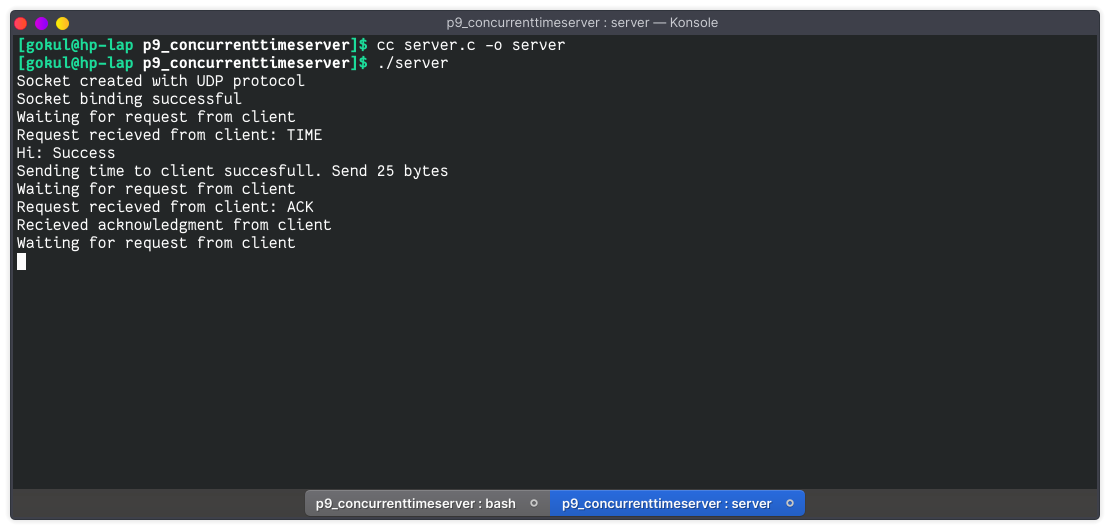
\includegraphics[width=0.90\textwidth]{img/p10/ss1.png}
	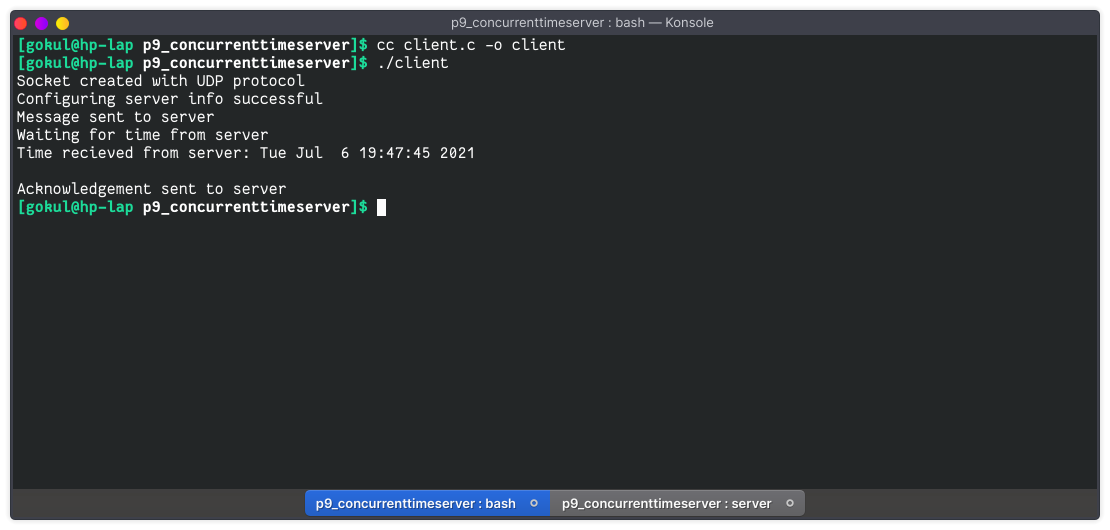
\includegraphics[width=0.90\textwidth]{img/p10/ss2.png}
\end{center}


\subsection{Result}
The above programs were executed and its output were verified

\end{document}